Codeigniter adalah sebuah framework untuk web yang dibuat dalam format PHP. Format yang dibuat ini selanjutnya dapat digunakan untu membuat sistem aplikasi web yang kompleks. Codeigniter dapat mempercepat proses pembuatan web, karena semua class dan modul yang dibutuhkan sudah ada dan programmer hanya tinggal menggunakannya kembali pada aplikasi web yang akan dibuat \cite{prabowo2015website}.

\section{Tutorial Install CodeIgniter 4}
\label{carainstallci4}
    \begin{enumerate}
        \item Kunjungi Link Resmi CodeIgniter di \textbf{\textit{"https://www.codeigniter.com/download"}}, kemudian pilih menu "View CodeIgniter 4 on Github".
		\begin{figure}[!htbp]
    		\centering
    		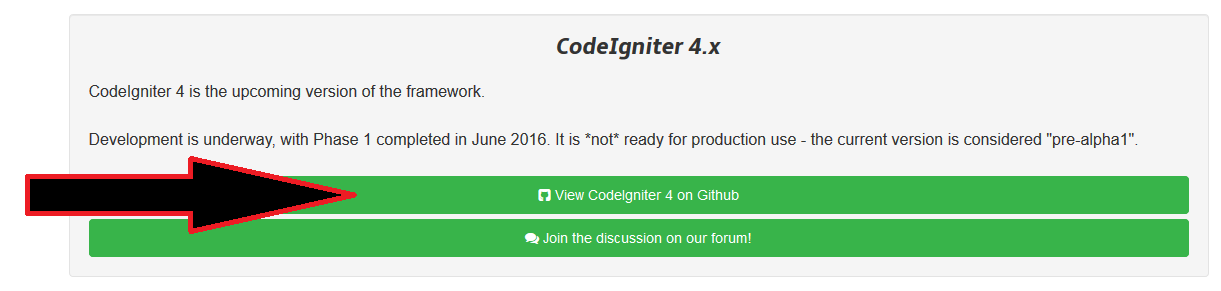
\includegraphics[width=0.9\textwidth]{figures/CODEIGNITER4/CI1_1.png}
    		\label{CodeIgniter1}
		\end{figure}
		
		\item Anda akan dibawa ke web github, dimana terdapat repository resmi untuk pengembangan Framework CodeIgniter 4, klik “Clone or download” kemudian “Download ZIP” untuk melakukan download Framework CodeIgniter 4.
		\begin{figure}[!htbp]
    		\centering
    		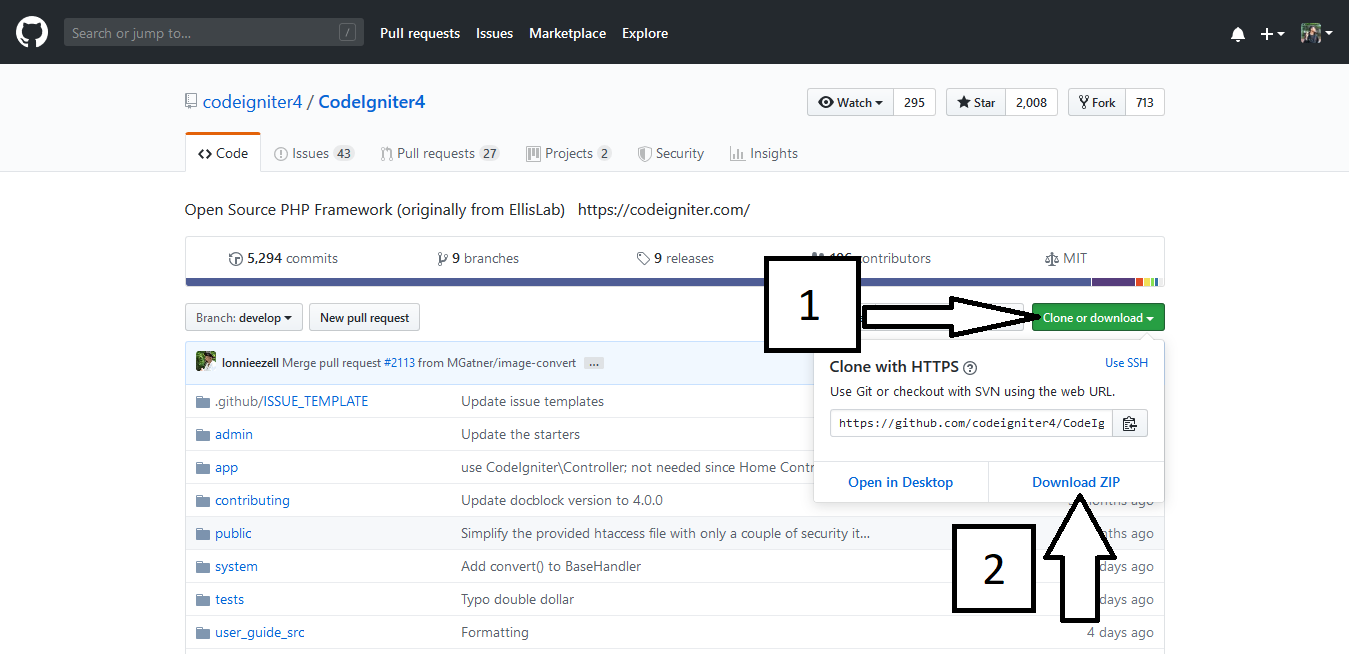
\includegraphics[width=0.5\textwidth]{figures/CODEIGNITER4/CI2.png}
    		\label{CodeIgniter2}
		\end{figure}
		
		\item Tunggu proses download sampai selesai, kemudian buka lokasi file yang didownload tadi dan copy file CodeIgniter4 ke dalam folder Xampp yang sudah di install sebelumnya di \verb|“C:\xampp7\htdocs”|.
		
		\item Extract file di folder tersebut, kemudian rename foldernya dengan nama aplikasi yang akan anda bangun, disini saya melakukan penamaan foldernya menjadi \verb|“ci4_leafletjs”|.
		\begin{figure}[!htbp]
    		\centering
    		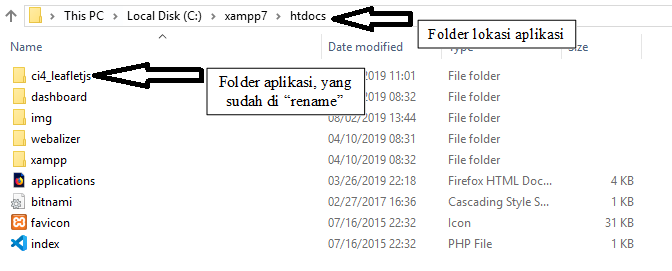
\includegraphics[width=0.5\textwidth]{figures/CODEIGNITER4/CI3.PNG}
    		\label{CodeIgniter3}
		\end{figure}
		
		\item Buka aplikasi \verb|“ci4_leafletjs”| dengan editor kesayangan anda, disini saya menggunakan visual studio code. Cara instal dan download bisa mengunjungi link berikut: \textbf{\textit{"https://code.visualstudio.com/download"}}.
		\begin{figure}[!htbp]
    		\centering
    		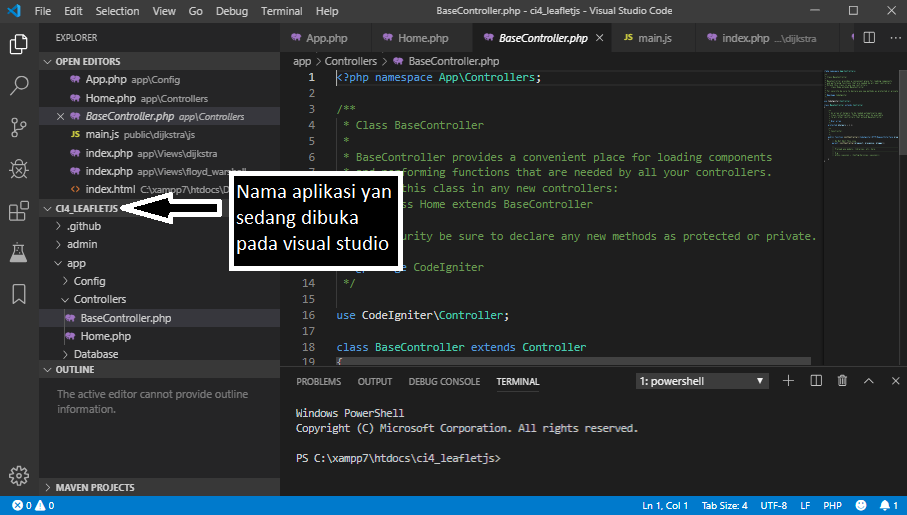
\includegraphics[width=0.5\textwidth]{figures/CODEIGNITER4/CI4.PNG}
    		\label{CodeIgniter4}
		\end{figure}
		
		\item Buka file App.php pada folder "app/Config/App.php", kemudian pada bagian \verb|"public $baseURL = ''"| diganti menjadi link aplikasi, sehingga seperti ini \verb|"public $baseURL = 'http://localhost:8080/';"|.
		\begin{figure}[!htbp]
    		\centering
    		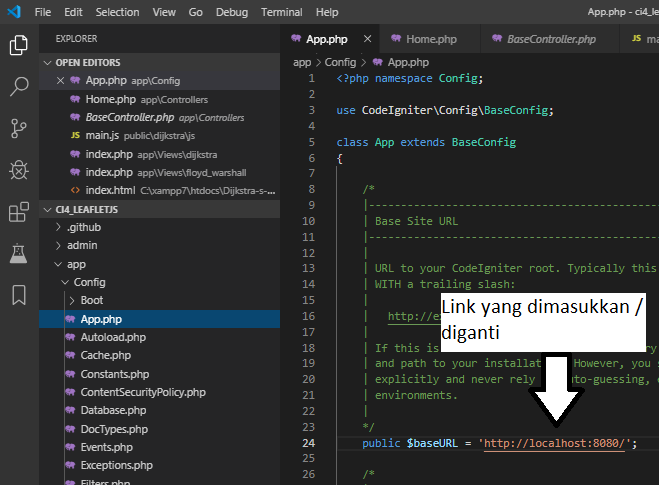
\includegraphics[width=0.5\textwidth]{figures/CODEIGNITER4/CI5.PNG}
    		\label{CodeIgniter5}
		\end{figure}
		
		\item CodeIgniter 4 sudah siap digunakan, jalankan aplikasi tersebut dengan cara berikut:
		\label{cararunci4}
		\begin{enumerate}
		    \item Klik menu Terminal yang ada pada menu bar atas Visual Studio Code, kemudian klik New Terminal atau bisa dengan cara menekan "Ctrl + Shift + `" pada keyboard anda. Setelah itu akan muncul terminal dibagian bawah pada Visual Studio Code seperti pada gambar berikut:
    		\begin{figure}[!htbp]
        		\centering
        		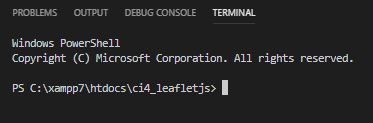
\includegraphics[width=0.5\textwidth]{figures/CODEIGNITER4/CI6.PNG}
        		\label{CodeIgniter6}
    		\end{figure}
    		
    		\item Masuk ke dalam folder public dengan cara mengetikkan "cd public" pada terminal.
    		\begin{figure}[!htbp]
        		\centering
        		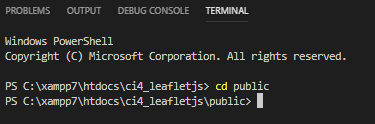
\includegraphics[width=0.5\textwidth]{figures/CODEIGNITER4/CI7.PNG}
        		\label{CodeIgniter7}
    		\end{figure}
    		
    		\item Ketikkan "php -S localhost:8080" pada terminal sehingga terlihat seperti pada gambar berikut:
    		\begin{figure}[!htbp]
        		\centering
        		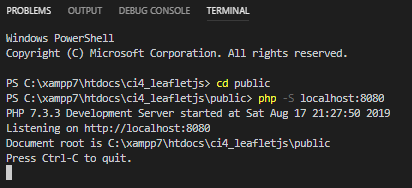
\includegraphics[width=0.5\textwidth]{figures/CODEIGNITER4/CI8.PNG}
        		\label{CodeIgniter8}
    		\end{figure}
    		
    		\item Bisa juga menggunakan cara kedua yaitu dengan mengetikkan "php spark serve" pada terminal sehingga terlihat seperti pada gambar berikut:
    		\begin{figure}[!htbp]
        		\centering
        		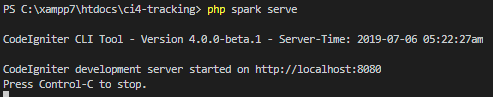
\includegraphics[width=0.5\textwidth]{figures/CODEIGNITER4/CI8_1.PNG}
        		\label{CodeIgniter9}
    		\end{figure}
    		
    		\item Jalankan aplikasi \verb|ci4_leafletjs| anda pada browser kesayangan anda, dengan cara mengetikkan "localhost:8080".
    		\begin{figure}[!htbp]
        		\centering
        		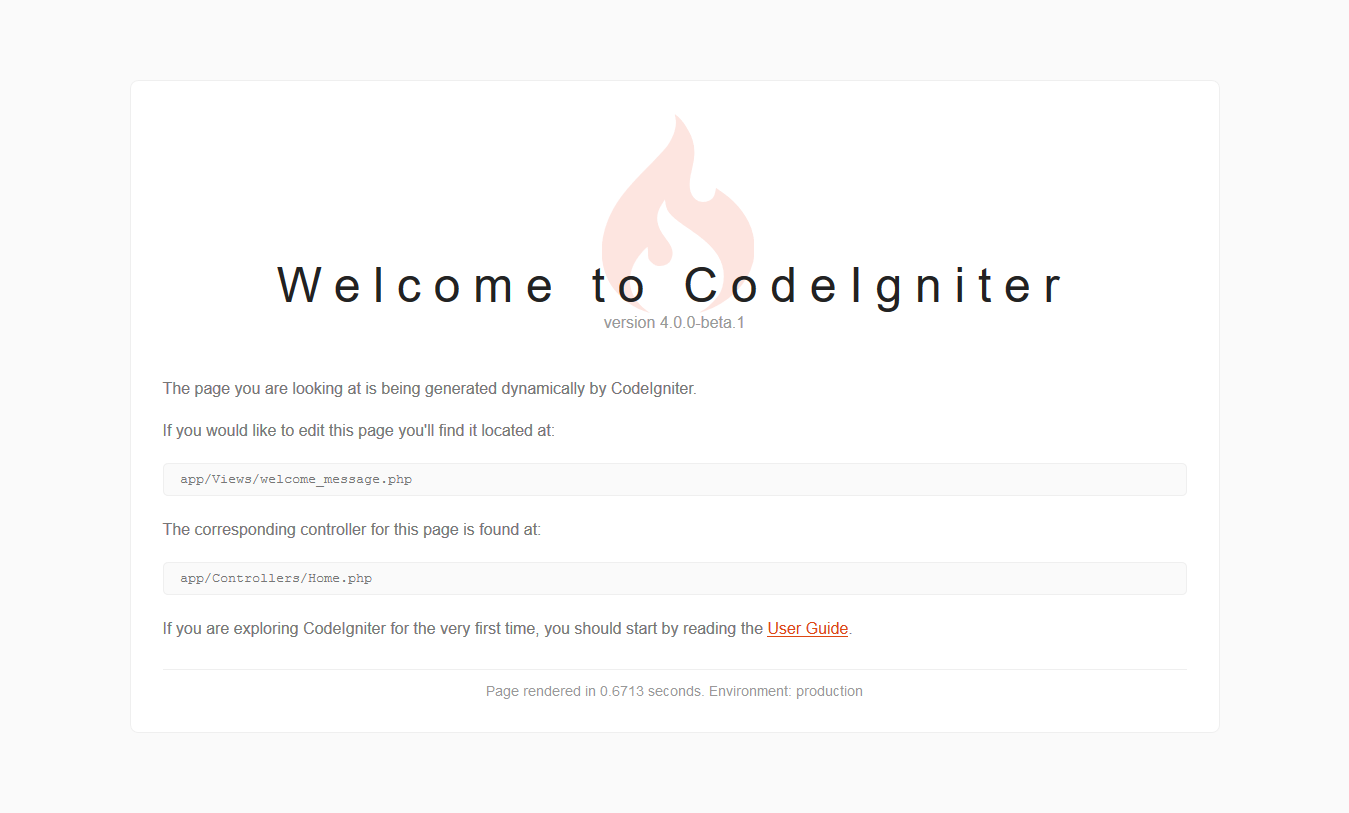
\includegraphics[width=0.8\textwidth]{figures/CODEIGNITER4/CI9.png}
        		\label{CodeIgniter10}
    		\end{figure}
    		
    		\item Kenapa "localhost:8080"? karena CodeIgniter 4 dilengkapi dengan server pengembangan lokal, memanfaatkan server web bawaan PHP dengan perutean CodeIgniter. Untuk info lebih jelasnya dapat dilihat pada link \textbf{\textit{"https:/ /codeigniter4.github.io/userguide/installation/running.html"}}.
		\end{enumerate}
    \end{enumerate}
    
    
    
    
    
\section{Konfigurasi CodeIgniter 4}
Di dalam folder config pada CodeIgniter terdapat berbagai macam file konfigurasi yang dapat kita atur sendiri nantinya. File tersebut dapat ditemukan pada folder \verb|C:/xampp7/htdocs/ci4_leafletjs/app/Config/|. Untuk codeigniter 4 default konfigurasi bisa dilakukan pada 3 file yaitu, file App.php, Database.php dan Routes.php. Berikut cara konfigurasinya:
\begin{enumerate}
    \item \textbf{App.php}, digunakan untuk membuat pengaturan dasar untuk web app codeigniter anda, seperti \verb|base_url|, index page, cookie, proxy dan lain lain. Configurasi pada file ini dapat dilakukan sama seperti pada configurasi sebelumnya di section 2.1
    \item \textbf{Database.php}, digunakan untuk mengatur koneksi web app kita ke database. Pada database.php konfigurasi yang dilakukan untuk mengkoneksikan database yaitu MySQL dengan aplikasi web berbasis framework CodeIgniter.
    \item \textbf{Routes.php}, digunakan untuk mengatur default controller dan overide 404.
\end{enumerate}





\section{Konfigurasi Template CodeIgniter 4}
Ada berbagai macam konfigurasi template terhadap CodeIgniter, baik secara install maupun dengan cara konfigurasi sendiri. Pada tutorial kali ini saya ingin menerapkan bootstrap dan template di CodeIgniter dengan cara cepat. Untuk yang ingin menggunakan cara instan, bisa dengan cara mengunjungi website \textit{w3layout.com} dan website yang menyediakan assets template dan bootstrap siap pakai. Sedikit berbeda dengan codeigniter 3 yang dimana harus dibuatkan folder assets terlebih dahulu, untuk codeigniter 4 semua assets akan ditampung dalam satu folder yaitu folder public, dapat di temukan pada folder \verb|C:\xampp7\htdocs\ci4_leafletjs\public|, berikut cara konfigurasi template pada codeigniter 4:
\begin{enumerate}
    \item Siapkan template atau bootstrap yang sudah didownload
    \item Extrak file tersebut jika dalam bentuk .rar atau .zip
    \item Copy file hasil extrak tadi ke dalam folder public.
		\begin{figure}[!htbp]
    		\centering
    		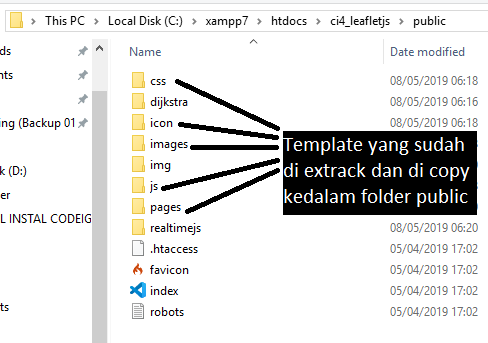
\includegraphics[width=0.5\textwidth]{figures/CODEIGNITER4/CI10.PNG}
    		\label{CodeIgniter11}
		\end{figure}
		
	\item Setelah menkopi file kedalam folder public, langka selanjutnya adalah memanggil config tersebut. Jangan lupa untuk membuat header dan footer ketika membuat website guna untuk mempermudah apabila terjadi perubahan terhadap beberapa menu.
	\item Copy isi dari index.html yang ada dalam template kemudian buat file di dalam folder \verb|C:/xampp7/htdocs/ci4_leafletjs/app/|views/agoritma/ index.php dengan format .php dan pastekan dalam file tersebut.
	\item Pertama lakukan konfigurasi terhadap index.php dengan cara memanggil link dan script yang sudah di copy di dalam folder public, berikut contoh pemanggilanya:
\begin{lstlisting}[caption=Konfigurasi Template di CodeIgniter 4]
<!DOCTYPE html>
<html lang="en">

<head>
    <meta charset="utf-8">
    <meta name="viewport" content="width=device-width, initial-scale=1.0, user-scalable=0, minimal-ui">
    <meta http-equiv="X-UA-Compatible" content="IE=edge" />
    <meta name="description" content="CodedThemes">
    <meta name="keywords" content=" Admin , Responsive, Landing, Bootstrap, App, Template, Mobile, iOS, Android, apple, creative app">
    <meta name="author" content="CodedThemes">

    <title>Dijkstra's Algorithm and Floyd-Warshall Algorithm</title>
  
    <link rel="icon" type="image/png" href="/images/favicon-32x32.png" sizes="32x32" />
    <link rel="icon" type="image/png" href="/images/favicon-16x16.png" sizes="16x16" />
    <link rel="icon" href="/images/favicon.ico" type="image/x-icon">
    <link rel="stylesheet" type="text/css" href="/css/bootstrap/css/bootstrap.min.css">
    <link rel="stylesheet" type="text/css" href="/css/datatables.css">
    <link rel="stylesheet" type="text/css" href="/css/buttons.dataTables.min.css">
    <link rel="stylesheet" type="text/css" href="/css/select2.css">
    <link rel="stylesheet" type="text/css" href="/css/style.css">
    <link rel="stylesheet" type="text/css" href="/css/style-bulog.css">
    <link rel="stylesheet" type="text/css" href="/css/style-bulog-print.css" media="print">
    <link rel="stylesheet" type="text/css" href="/css/jquery.mCustomScrollbar.css">
    <script type="text/javascript" src="/js/jquery/jquery.min.js"></script>
</head>
<body>
.....
    <div class="pcoded-content">
      <div class="pcoded-inner-content">
        <div class="main-body">
          <div class="page-wrapper">
            <div class="page-header card">
              <div class="row align-items-start">
                <div class="col-lg-8">
                  <div class="page-header-title">        
                    &copy; Faisal Syarifuddin <?php echo date('Y') ?>
                    <br>CodeIgniter Version <?= CodeIgniter\CodeIgniter::CI_VERSION ?>
                  </div>
                </div>
              </div>
            </div>
          </div>
        </div>
      </div>
    </div>
  </div>
  <script type="text/javascript" src="/js/script.js"></script>
</body>
</html>
\end{lstlisting}
		\par Lakukan pemanggilan terhadap semua code yang berbau href dan src, seperti pada codingan diatas. Setelah itu simpan.
		
	\item Pemanggilan template sudah selesai, jalankan aplikasi seperti pada cara yang sudah diterapakan sebelumnya di subbab \ref{carainstallci4}, maka akan muncul tampilan seperti gambar berikut:
		\begin{figure}[!htbp]
    		\centering
    		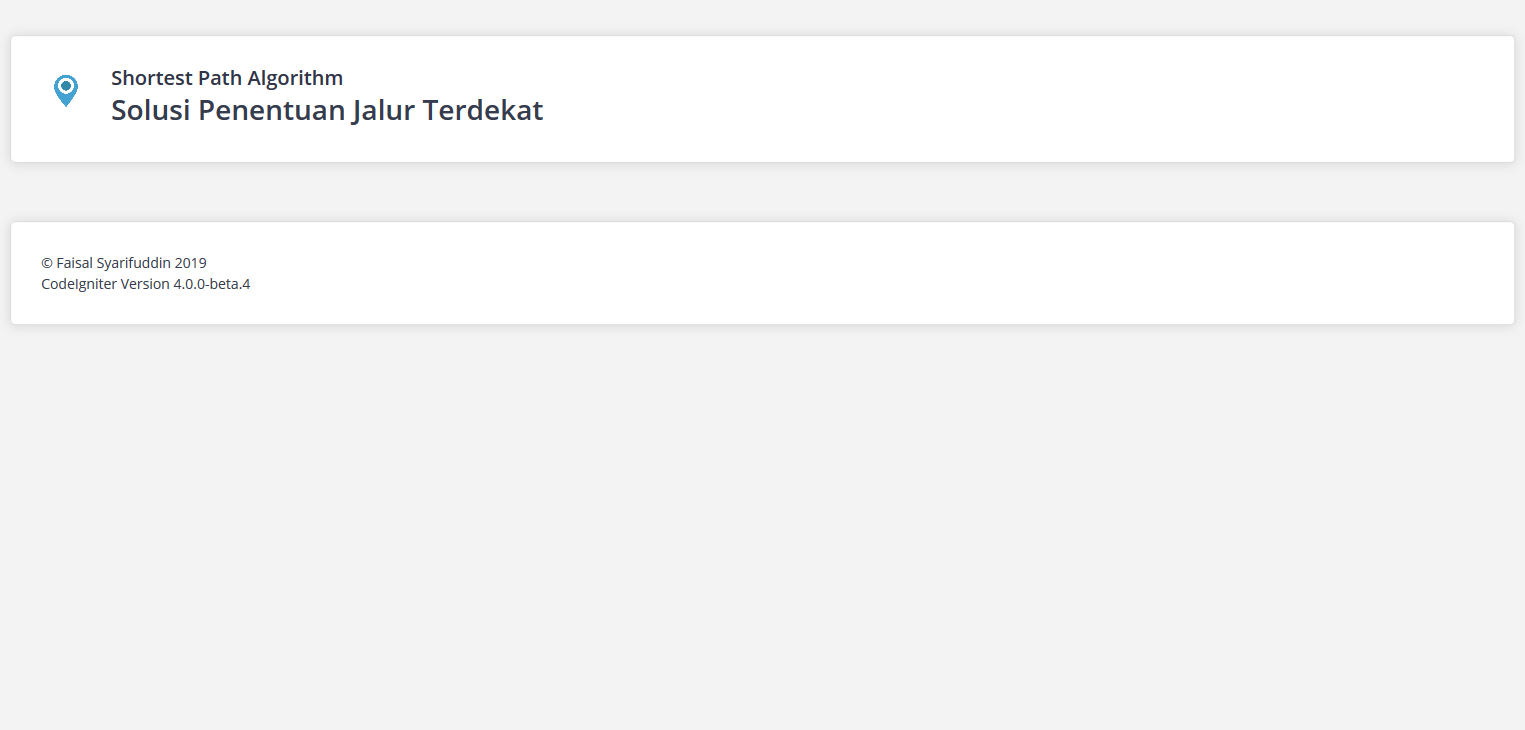
\includegraphics[width=0.8\textwidth]{figures/CODEIGNITER4/CI11.png}
    		\label{CodeIgniter12}
		\end{figure}
\end{enumerate}